\renewcommand{\baselinestretch}{1.0}
\chapter{Integration of behaviors: Obstacle Avoidance and Target Acquisition (nonlinear)}%
\label{ch:obstacle-target-nonlinear}
\renewcommand{\baselinestretch}{1.5}
In this chapter the obstacle avoidance and target acquisition behaviors are
integrated, but for the latter is considered a nonlinear dynamic system. A
detailed analysis is then performed over: obstacle avoidance and target
acqusition time constant precedence and tuning; distance between obstacles and
respective bifurcation analysis; the influence of noise (stochastic force). 
Finally, more demanding scenarios are simulated, respectively in \emph{S} or
\emph{U} shape, and the robot's behavior is analyzed.

\section{Implementation}
The nonlinear dynamic system that controls the movement of the robot for target
acquisition in a collision-free path is obtained
through the sum of the obstacles and target dynamic systems contribuitions and
also a stochastic component for escaping repellers in a finite time, as given by Eq.~(\ref{eq:36}):
%
\begin{equation}
\label{eq:36}
 \frac{d \phi}{dt} = \sum_{i = 1}^N{f_{obs,i}(\phi)} + f_{tar}(\phi) + f_{stoch}
\end{equation}

Thus, the implementation is simply the sum of these components (see Listing~\ref{lst:program-dyn-obs-tar-nonlinear}).
% program_dyn_tar.m (generic)
\lstinputlisting[language=matlab, caption={Implementation of obstacle
  avoidance behavior and target acquisiton},label=lst:program-dyn-obs-tar-nonlinear,
style=custom-matlab]{./listing/program_dyn_obs_tar_nonlinear.m}%

However, as it will be discussed further ahead, the tuning of the overall system
parameters is critical for adequate collision-free navigation to the target. By
design, the obstacle avoidance behavior takes precedence over target
acquisition, as obviously, in a limit case --- e.g., where the target is behind an
obstacle --- the robot must circumvent the obstacle, instead of hitting it. This
is guaranteed by imposing higher magnitude for repulsive component than for
attractive one, i.e. $\lambda_{obs} \gg \lambda_{tar}$, and consequently,
$\tau_{obs} \ll \tau_{tar}$.

\section{Scenario 1}%
\label{obst-tar-nonlinear-scenario1}
In this section are analyzed the influences of varying the magnitude of
attraction to target, $\lambda_{tar}$, the distance between obstacles, and the noise
(stochastic force) in the robot's navigation behavior.

\subsection{Magnitude of attraction to target: $\lambda_{tar}$}%
\label{obst-tar-nonlinear-lambda-tar}
If the magnitude of the target is greater than the obstacles, the
issue that occurs is that it is only when the robot is a very short distance
from the obstacle that the repeller is established. When the robot is close to
the obstacle this one is detected in several directions and the sum of these
repulsive forces exceeds the force of attraction, changing the stability of the
fixed point of that navigation direction (Fig~\ref{fig:obs-tar-nonlinear-different-lambda}).
%
\begin{figure}[htb!]
  \centering
  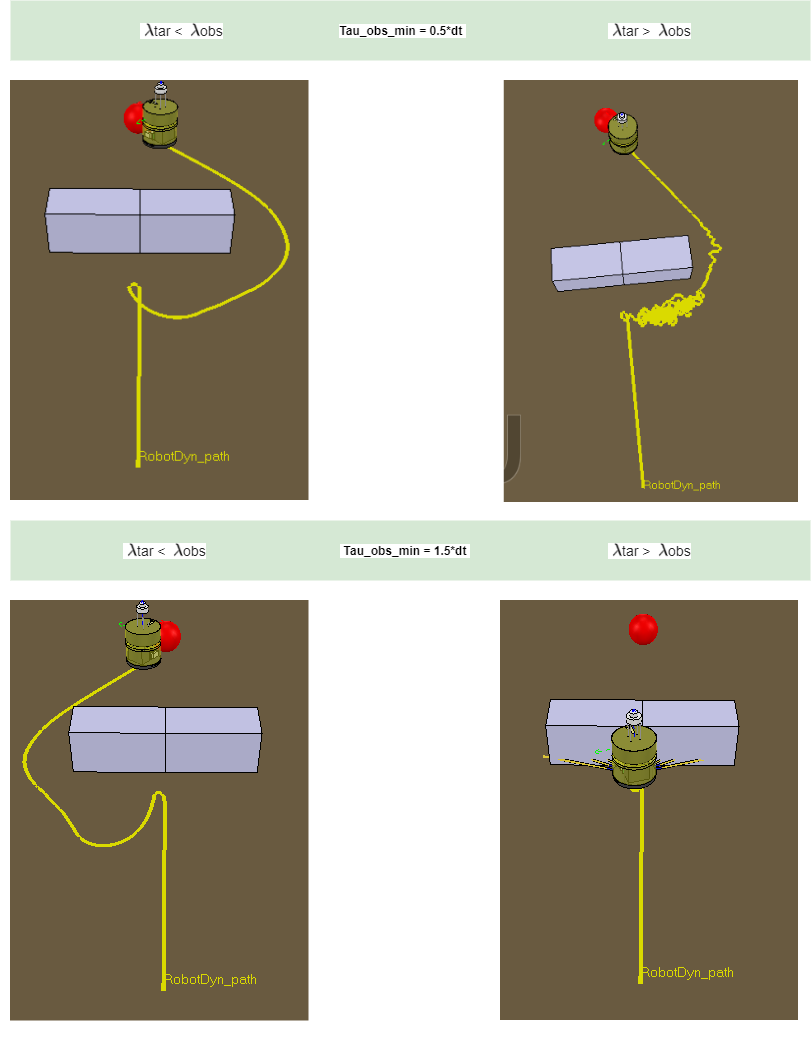
\includegraphics[width=0.6\textwidth]{img/ytar.png}
  \caption{Different $\lambda_{tar}$ values simulations results.}%
  \label{fig:obs-tar-nonlinear-different-lambda}
\end{figure}

Consequently, as shown in Fig.~\ref{fig:obs-tar-nonlinear-different-lambda}, or the robot collides with the obstacle or has a very irregular route, depending on the time constant. Having enough time to escape the repeller, the robot has a zigzag route, because it approaches the obstacle and moves away successively since it is only close to this that it realizes that there is an obstacle. If there is not enough time to change the heading direction, the robot collides.
Therefore, the magnitude of the repulsing from the obstacle must always be
greater than that of the attraction to
the target, i.e., 
$\lambda_{obs} \gg \lambda_{tar}$, and consequently, $\tau_{obs} \ll \tau_{tar}$.
%
\subsection{Different gaps between obstacles}
In this scenario, \texttt{MobileRobotDyn\_Tar\_Obs.ttt},
several simulations are performed for different gaps between obstacles, namely 0
cm, 10 cm and 50 cm span.

\subsubsection{No gap (0 cm)}%
\label{sec:Different-gaps-0cm}
Fig.~\ref{fig:obs-tar-nonlinear-behavioral} illustrates the simulations
performed for obstacles forming a wall without gap (0 cm).
%
\begin{figure}[htb!]
  \centering
  \begin{subfigure}{.45\textwidth}
  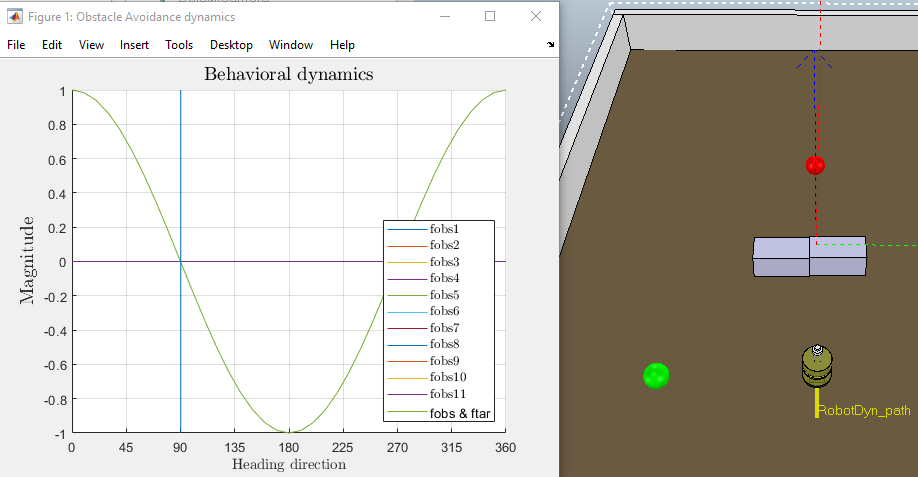
\includegraphics[width=\textwidth]{img/3-2-1.PNG}%
  \caption{}%
  \label{fig:obs-tar-nonlinear-behavioral-1}
  \end{subfigure}
  \begin{subfigure}{.45\textwidth}
    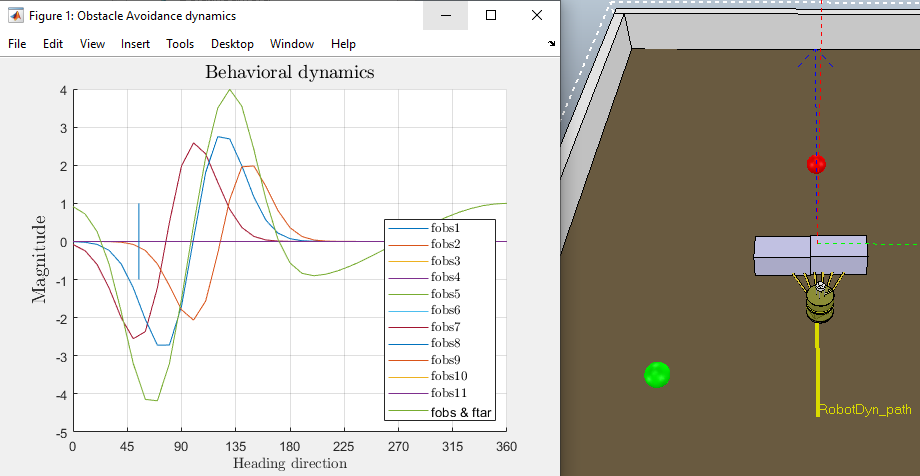
\includegraphics[width=\textwidth]{img/3-2-2.PNG}%
  \caption{}%
  \label{fig:obs-tar-nonlinear-behavioral-2}
  \end{subfigure}
  % 
  \begin{subfigure}{.45\textwidth}
    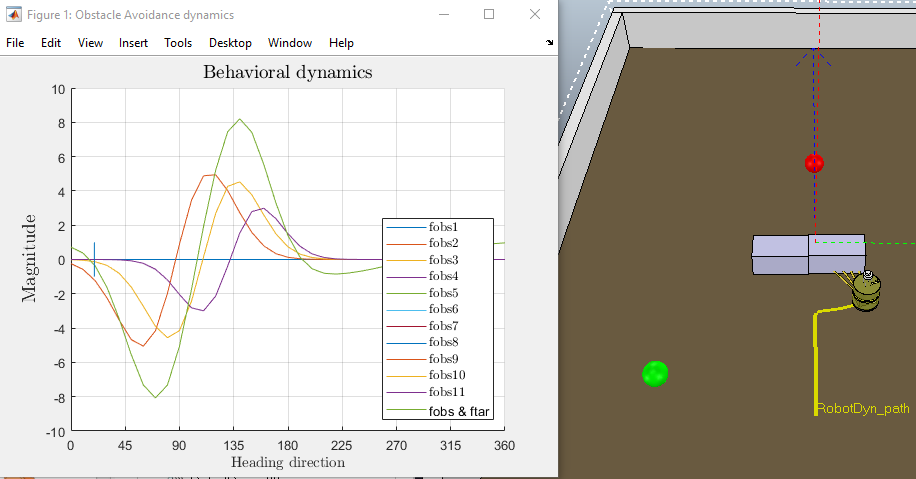
\includegraphics[width=\textwidth]{img/3-2-3.PNG}%
  \caption{}%
  \label{fig:obs-tar-nonlinear-behavioral-3}
  \end{subfigure}
  % 
  \begin{subfigure}{.45\textwidth}
    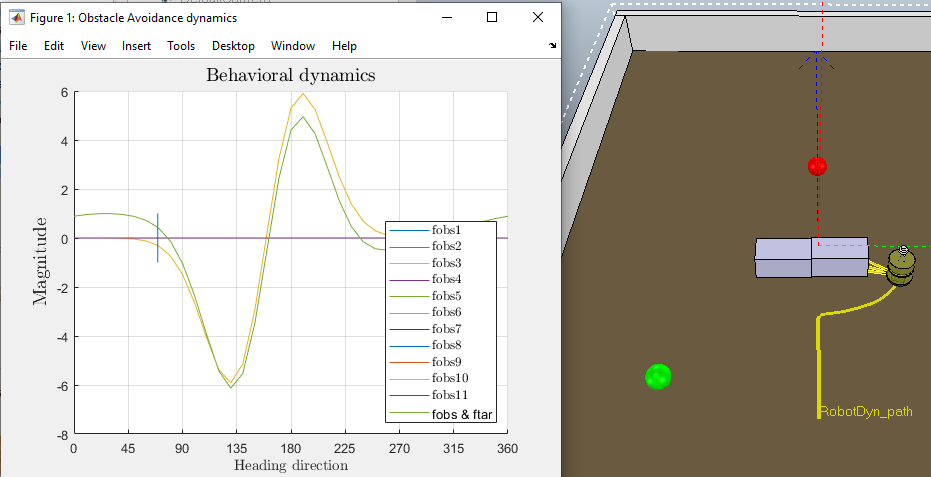
\includegraphics[width=\textwidth]{img/3-2-4.PNG}%
  \caption{}%
  \label{fig:obs-tar-nonlinear-behavioral-4}
  \end{subfigure}
  \begin{subfigure}{.45\textwidth}
    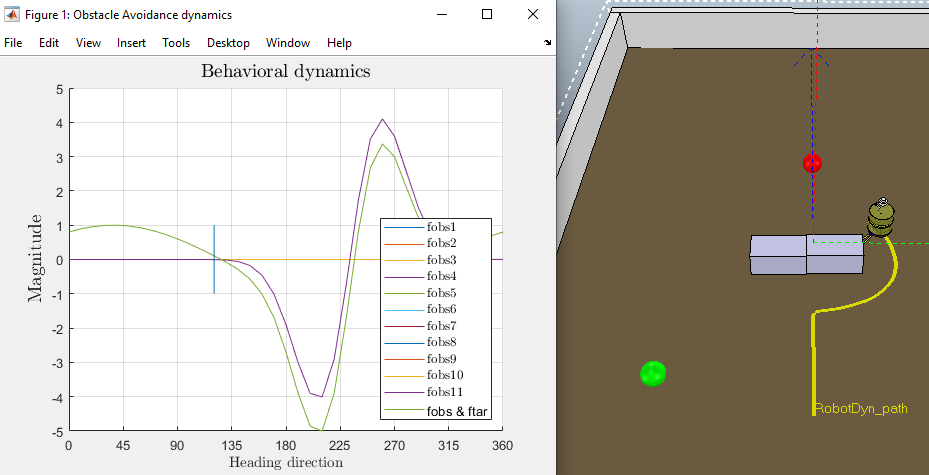
\includegraphics[width=\textwidth]{img/3-2-5.PNG}%
  \caption{}%
  \label{fig:obs-tar-nonlinear-behavioral-5}
  \end{subfigure}
  % 
  \begin{subfigure}{.45\textwidth}
    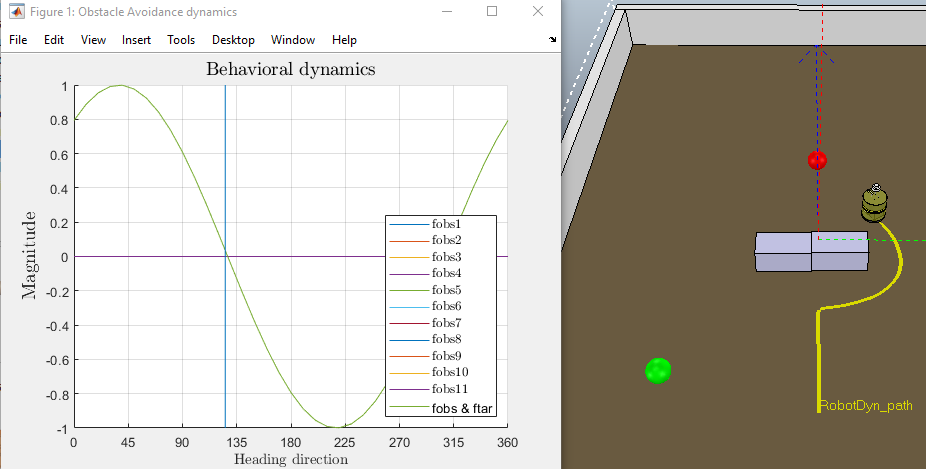
\includegraphics[width=\textwidth]{img/3-2-6.PNG}%
  \caption{}%
  \label{fig:obs-tar-nonlinear-behavioral-6}
  \end{subfigure}
  \caption{Behavioral Dynamics depending on the robot's position in the world}%
  \label{fig:obs-tar-nonlinear-behavioral}
\end{figure}

In the first simulation, the obstacles form a wall and the robot is
positioned in front of the obstacles but without the sensors detecting it. (Fig.~\ref{fig:obs-tar-nonlinear-behavioral-1}). 
The stochastic force is not considered and the parameter $\beta _{2}$ is 50.
In the initial moments, obstacles are not detected by the sensors, so they do
not contribute to the dynamics vector field in the navigation direction 
positioned in front of the obstacles but without the sensors detected.

As the robot approaches the wall, the sensors begin to detect obstacles, in the
first moments, due to the considerable distance to the obstacle, the repeller is
of low magnitude so it does not prevail, therefore an attractor is formed in the
direction of navigation, with a lower intensity of attraction than
before. However, as the distance to the obstacles decreases, it is visible that
the intensity of the repeller increases and dominates, an instability occurs,
the vector field of the dynamics of the navigation direction starts to have a
repeller in that direction. When the stability of the fixed points changes, it
because the bifurcation point has been exceeded, and the robot will present a
different behaviour than previous.

So such behavior is in line with expectations since with the proximity to an
obstacle the forces of repulsion
appear and prevail over attraction forces. Because of that the robot can escape from the obstacle to the right or
left, because there are two attractors in these directions, attending at the
Figs.~\ref{fig:obs-tar-nonlinear-behavioral-2} to~\ref{fig:obs-tar-nonlinear-behavioral-5}, it can be noted, the heading direction of the robot
converges to one of the attractors. In this simulation episode, the robot moves
to the right to avoid a collision with the wall. 

When the obstacle is surpassed, it is no longer detected by the sensors, the
repulsion forces sum is zero, so they no longer contribute to the vector
field. Because of that, there is an attractor in the direction of the target,
and this is where the robot progresses successfully. Once again, the robot's
behavioral dynamics changed.
(Fig.~\ref{fig:obs-tar-nonlinear-behavioral-6}). 

\subsubsection{10 cm}%
\label{sec:Different-gaps-10cm}
In the second simulation, the obstacles are 10 cm apart and the robot is
positioned in front of the obstacles but without the sensors detecting them, as
illustrated in Fig.~\ref{fig:obs-tar-nonlinear-behavioral-10}. 
The stochastic force is not considered, the parameter $\beta _{2}$ is 50.
%
\begin{figure}[htb!]
  \centering
  \begin{subfigure}{.45\textwidth}
    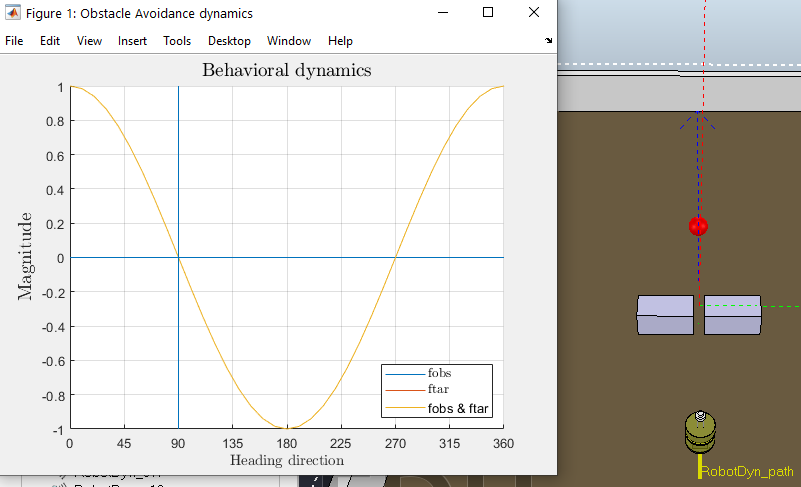
\includegraphics[width=\textwidth]{img/3-2-3-1.PNG}
    \caption{}%
    \label{fig:obs-tar-nonlinear-behavioral-10-1}
  \end{subfigure}
  % 
  \begin{subfigure}{.45\textwidth}
    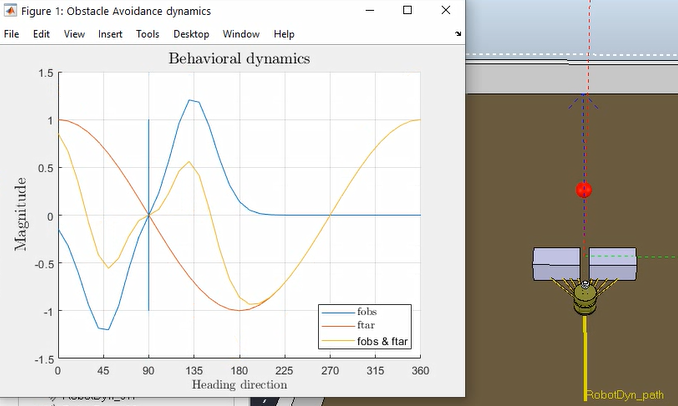
\includegraphics[width=\textwidth]{img/3-2-3-2.PNG}
    \caption{}%
    \label{fig:obs-tar-nonlinear-behavioral-10-2}
  \end{subfigure}
  % 
    \begin{subfigure}{.45\textwidth}
      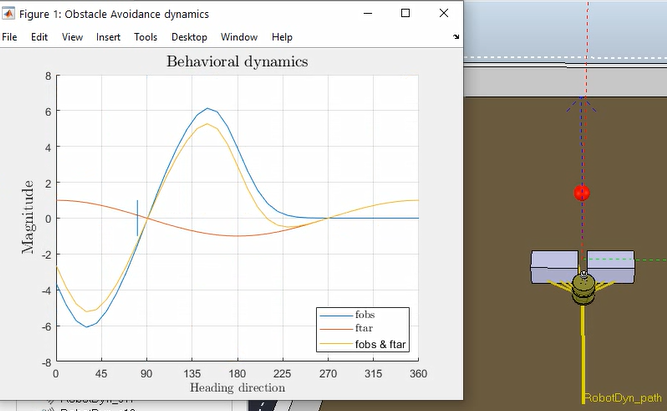
\includegraphics[width=\textwidth]{img/3-2-3-3.PNG}
    \caption{}%
    \label{fig:obs-tar-nonlinear-behavioral-10-3}
    \end{subfigure}
%
    \begin{subfigure}{.45\textwidth}
      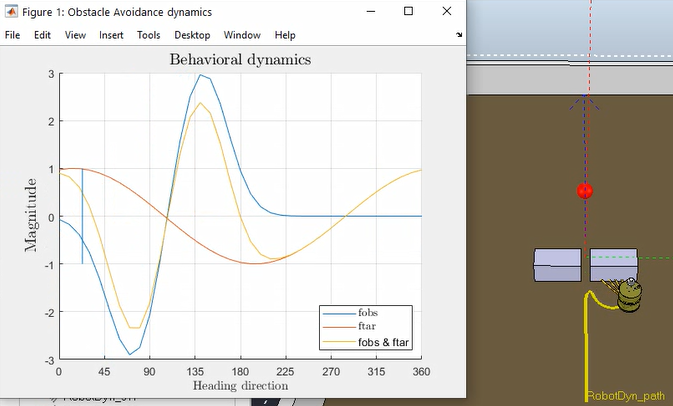
\includegraphics[width=\textwidth]{img/3-2-3-4.PNG}
    \caption{}%
    \label{fig:obs-tar-nonlinear-behavioral-10-4}
    \end{subfigure}
%
    \begin{subfigure}{.45\textwidth}
      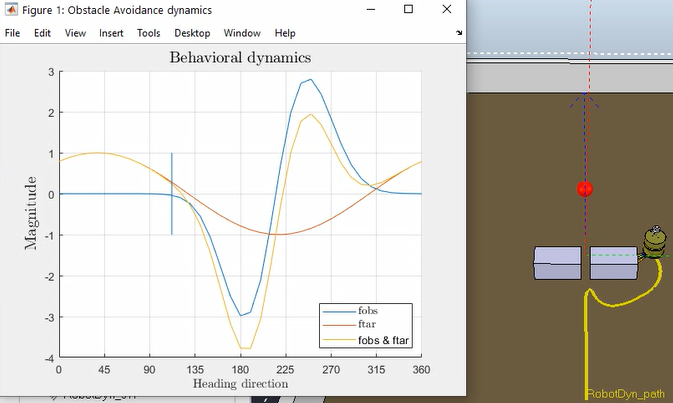
\includegraphics[width=\textwidth]{img/3-2-3-6.PNG}
    \caption{}%
    \label{fig:obs-tar-nonlinear-behavioral-10-5}
    \end{subfigure}
    % 
    \begin{subfigure}{.45\textwidth}
      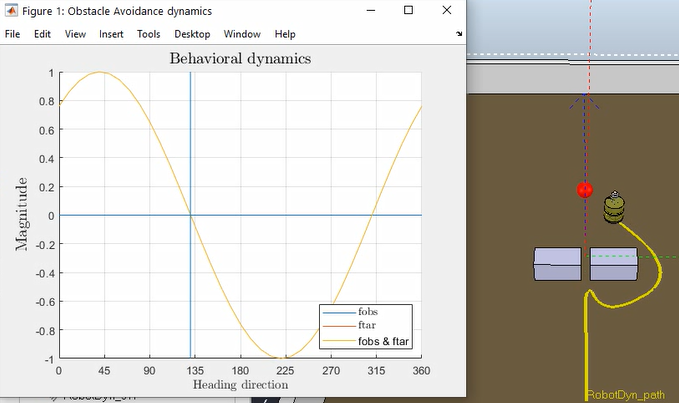
\includegraphics[width=\textwidth]{img/3-2-3-7.PNG}
    \caption{}%
    \label{fig:obs-tar-nonlinear-behavioral-10-6}
    \end{subfigure}
    \caption{Behavioral Dynamics depending on the robot's position in the world for a 10 cm gap}%
    \label{fig:obs-tar-nonlinear-behavioral-10}
  \end{figure}

In Fig.~\ref{fig:obs-tar-nonlinear-behavioral-10-1} the sensors have not yet
detected obstacles, so only the target contributes to the vector field, yielding
an attractor in the forward heading direction. The robot proceeds. As the
robot approaches the obstacles, the repulsion forces present greater magnitude,
and therefore dominate, yielding a repeller in the heading direction of 90
degrees, and more, two attractors are erected, one on the left and one on the
right, giving two escape routes for the robot so that there is no collision with
the obstacles. It is in this situation that the behavior change occurs ---
the fixed point for the heading direction was asymptotically stable and now
becomes unstable, causing the robot to turn, in this case, to the
right (see Figs.~\ref{fig:obs-tar-nonlinear-behavioral-10-2} and~\ref{fig:obs-tar-nonlinear-behavioral-10-3}).

Figs.~\ref{fig:obs-tar-nonlinear-behavioral-10-4} and~\ref{fig:obs-tar-nonlinear-behavioral-10-5} show, through the diagram, that the robot progresses in the
direction of one of the attractors, and through the simulation environment, it
is seen that the robot bypasses the obstacle without collisions, because the
vector field continues with a repeller in the direction of the obstacles. With
the movement towards the attractor, the heading direction of the robot meets
the target, as desired.
%
\subsubsection{50 cm}%
\label{sec:Different-gaps-50cm}
In the last simulation, the obstacles are 50 cm apart and the robot is
positioned in front of the obstacles but without the sensors detecting them as
illustrated in Fig.~\ref{fig:obs-tar-nonlinear-behavioral-50}. 
The stochastic force is not considered and the $\beta _{2} = 50$.

\begin{figure}[htb!]
  \centering
%
  \begin{subfigure}{.45\textwidth}
  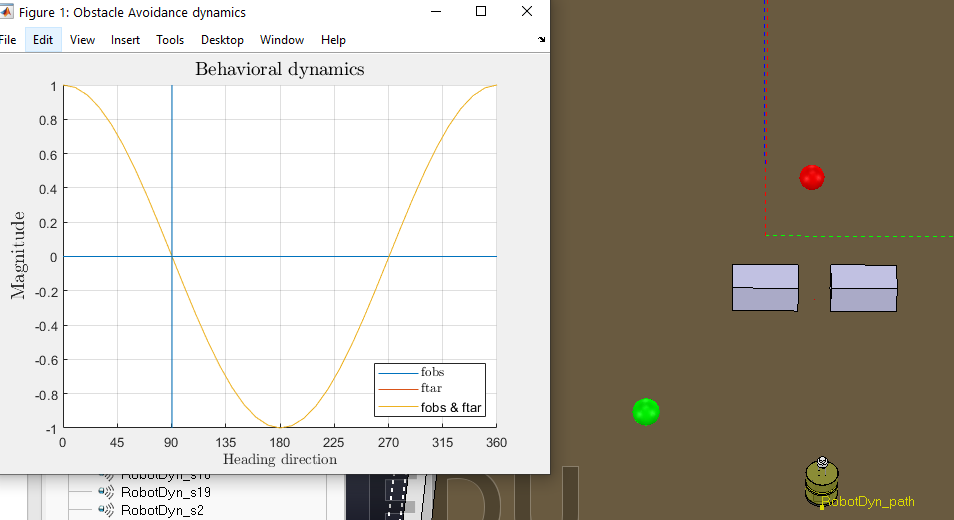
\includegraphics[width=\textwidth]{img/3-3-1.PNG}%
  \caption{}%
  \label{fig:obs-tar-nonlinear-behavioral-50-1}
  \end{subfigure}
%
  \begin{subfigure}{.45\textwidth}
    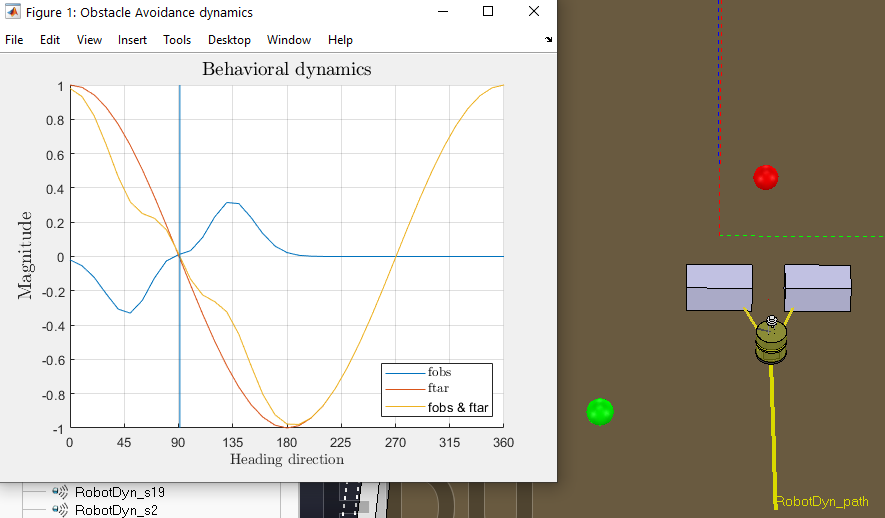
\includegraphics[width=\textwidth]{img/3-3-2.PNG}%
  \caption{}%
  \label{fig:obs-tar-nonlinear-behavioral-50-2}
  %  \caption{(b)}
  \end{subfigure}
%
  \begin{subfigure}{.45\textwidth}
    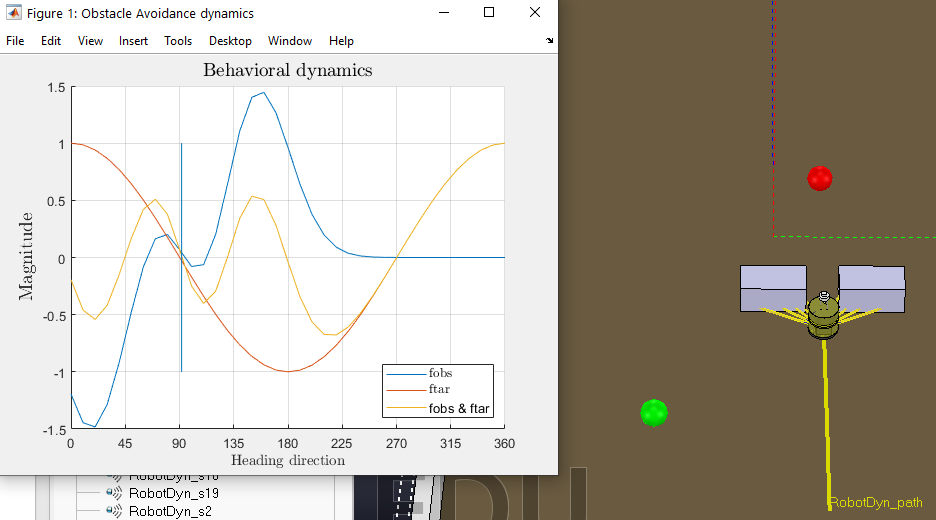
\includegraphics[width=\textwidth]{img/3-3-3.PNG}%
  \caption{}%
  \label{fig:obs-tar-nonlinear-behavioral-50-3}
  %  \caption{(c)}
  \end{subfigure}
  % 
  \begin{subfigure}{.45\textwidth}
    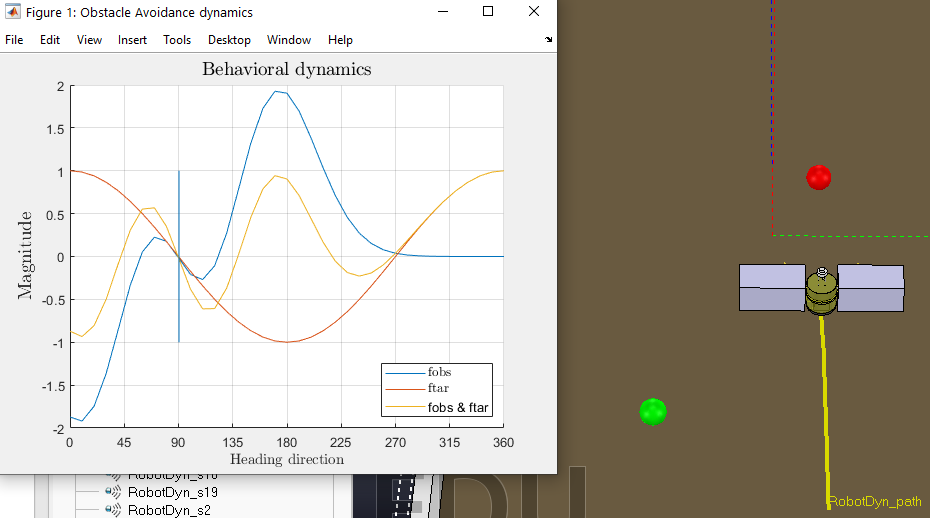
\includegraphics[width=\textwidth]{img/3-3-4.PNG}%
  \caption{}%
  \label{fig:obs-tar-nonlinear-behavioral-50-4}
  %  \caption{(d)}
  \end{subfigure}
%
  \begin{subfigure}{.45\textwidth}
  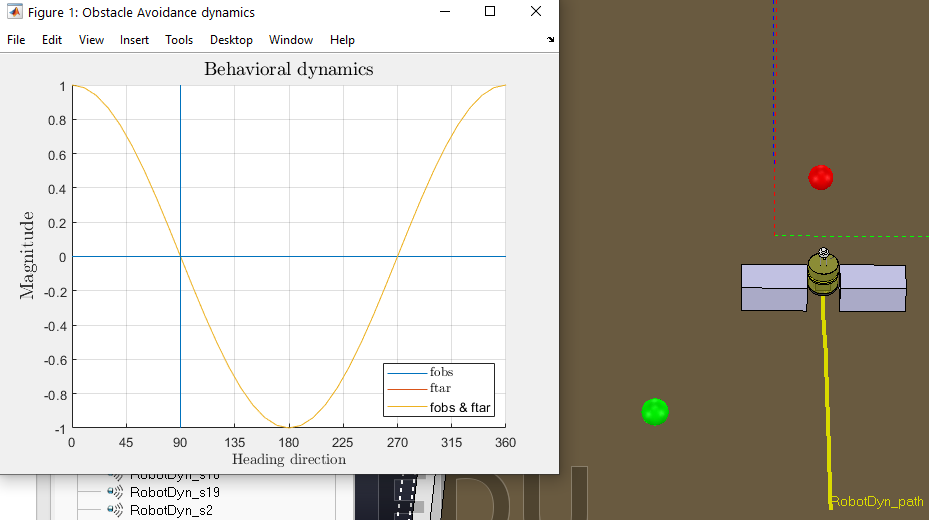
\includegraphics[width=\textwidth]{img/3-3-5.PNG}%
  \caption{}%
  \label{fig:obs-tar-nonlinear-behavioral-50-5}
  %\caption{(f)}
  \end{subfigure}
  \caption{Behavioral Dynamics depending on the robot's position in the world for a 50 cm gap}%
  \label{fig:obs-tar-nonlinear-behavioral-50}
\end{figure}

In the beginning (Fig.~\ref{fig:obs-tar-nonlinear-behavioral-50-1}), no obstacle
is detected --- the vector field of the dynamics of the heading direction is an attractor in the direction of the target.
As the robot continues forward, the target's contribution remains, with an
attractor in the 90-degree heading direction. In the first moments when the
robot's sensors detects obstacles (Fig.~\ref{fig:obs-tar-nonlinear-behavioral-50-2}), the sum
of its forces yields a repeller at 90 degrees, where an attractor already
exists, a contribution made by the target. It is clear by the figure that the
contribution made by the target has greater magnitude, so it dominates,
therefore in the heading direction of 90 degrees an attractor is
established. The robot proceeds forward.

With the proximity to the obstacles (Fig.~\ref{fig:obs-tar-nonlinear-behavioral-50-3}), it is increasingly noticeable that the
obstacles are spaced apart, so each contribution of the obstacles will be more
precise and, consequently, more distributed by the different degrees of heading
direction, because of this the sum of all
repulsion forces yields an attractor in the 90-degree navigation
direction. What coincides with the attractor built by the force of attraction,
the robot continues forward.

The vector field persists with this logic (Fig.~\ref{fig:obs-tar-nonlinear-behavioral-50-4}). When the robot overcomes
obstacles, the sum of these repulsive forces becomes null and insignificant for
the vector field (Fig.~\ref{fig:obs-tar-nonlinear-behavioral-50-5}).

\subsection{Influence of noise}%
\label{sec:obs-tar-nonlinear-noise}
To verify the contribution of noise, the robot was positioned at a short distance from the wall, in two episodes noise was considered (Q = 0.05 and Q = 0.5) and in another it was not taken into account (Q = 0).
It was found that in the situation in which the noise is added to the dynamics the robot manages to escape and avoid the obstacle, in the opposite situation the robot collided, illustrated in Fig.~\ref{fig:obs-tar-nonlinear-noise}.
This experiment reinforces the importance of adding noise to the dynamic system,
for when the robot is in a repeller be able to escape in a finite time. 
%
\begin{figure}[htb!]
  \centering
  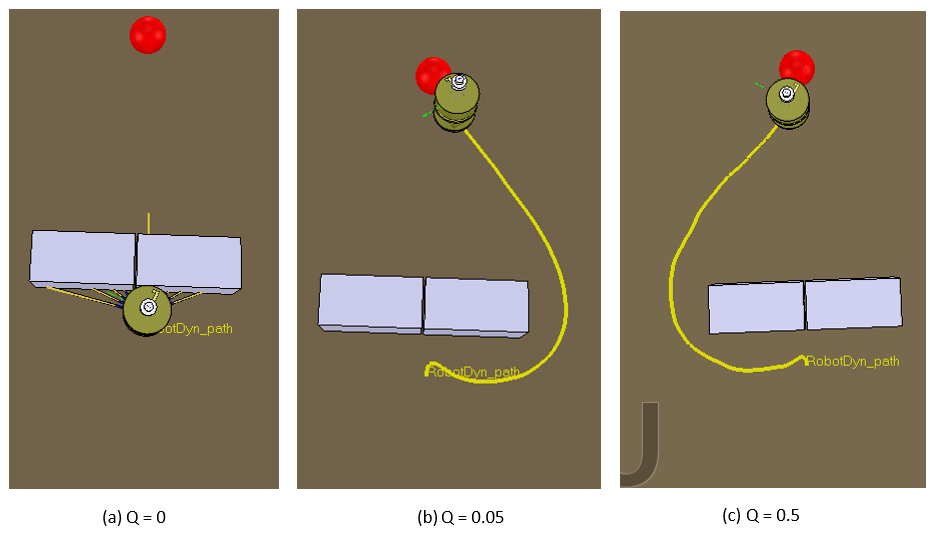
\includegraphics[width=0.7\textwidth]{img/obs-tar-nonlinear-noise.PNG}
  \caption{Simulation results for the overall dynamic field with different noise levels}%
  \label{fig:obs-tar-nonlinear-noise}
\end{figure}
%

In addition, comparing the two experiments in which the noise was added it is also possible to make conclusions. The trajectory that the robot does when Q = 0.05 is smoother than when Q = 0.5. 
That said, when choosing the values of Q, it must be taken into account that the value must ensure that the robot escapes to the repeller and does not make abrupt direction adjustments, so always give preference to small values.
Since the Gaussian white noise is a stochastic function, then the trajectory
taken by the robot --- the left or right attraction basin --- will be selected
in a probabilistic way by this function, contributes for behavioral diversity
when the robot must deviate from the obstacles, enabling it to turn left or right,
depending on the stochastic effect. 
%
\subsection{Scenario 2}
In this simulation is used the \texttt{MobileRobotDyn\_Tar\_Obs\_S.ttt}
scenario, an S-shape scenario, to demonstrate the overall dynamics robustness
for a more complex scenario. As can be observed (Fig.~\ref{fig:obs-tar-nonlinear-scenario2}), the robot is able to avoid obstacles and reach the target.

\begin{figure}[htb!]
  \centering
  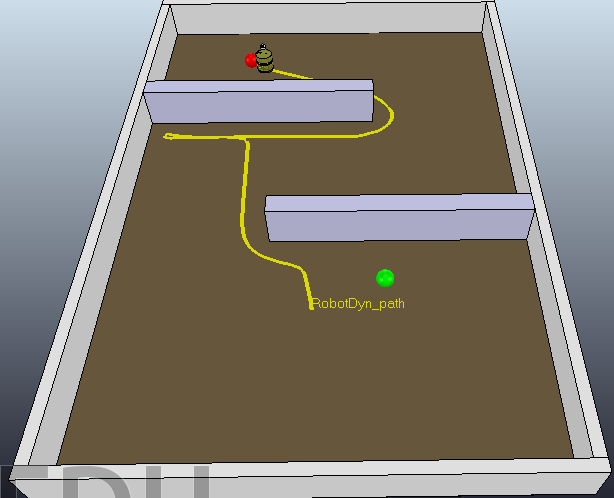
\includegraphics[width=0.8\textwidth]{img/mapa1.PNG}
  \caption{Simulation in the \texttt{MobileRobotDyn\_Tar\_Obs\_S.ttt} scenario}%
  \label{fig:obs-tar-nonlinear-scenario2}
\end{figure}

\subsection{Scenario 3}
In this simulation is used the \texttt{MobileRobotDyn\_Tar\_Obs\_U.ttt}
scenario, an U-shape scenario, to demonstrate the overall dynamics robustness
for an ever more complex scenario.
(see Fig.~\ref{fig:obs-tar-nonlinear-scenario3} and Video \href{run:./videos/obs-tar-nonlinear-Uscenario.mp4}{./videos/
obs-tar-nonlinear-Uscenario.mp4}). Once again, the robot is able to avoid obstacles and reach the target.
The behavior is the same as already described: in the presence of an obstacle,
a repeller is placed in that heading direction and two attractors,
representing the possible heading directions for the escape, only when these
forces are the most intense, which depends on the proximity to the
obstacle. When the sensors do not detect obstacles, only the force of attraction
to the target
contributes to the vector field of the heading direction.
%
\begin{figure}[htb!]
  \centering
  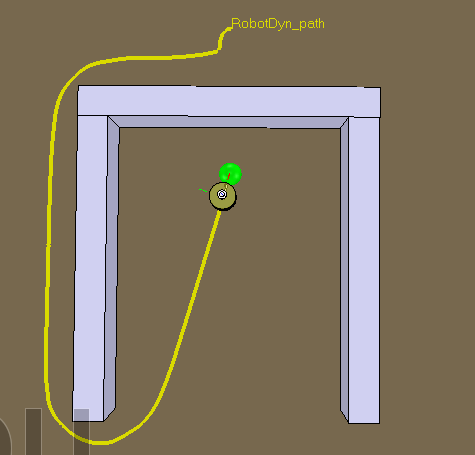
\includegraphics[width=0.7\textwidth]{img/mapa2.PNG}
  \caption{Simulation in the \texttt{MobileRobotDyn\_Tar\_Obs\_U.ttt} scenario}%
  \label{fig:obs-tar-nonlinear-scenario3}
\end{figure}

\subsection{Discussion}
In conclusion, the vector field of the navigation direction is constituted by
the attraction force and the sum of repulsion forces, with each force establishing an attractor and/or a repeller. With the movement of the robot around the world, it is expected that it will change its behavior in accordance with its surroundings. The decisions that the robot undertakes to navigate with a certain heading direction or to continue in it depends on the bifurcations.
Therefore, the stability of fixed points can change and other new fixed points
appear.

The obstacle avoidance behavior must take precedence over the target acquisition
to prevent the robot from hitting an obstacle while attempting to move to the
target. This is guaranteed by imposing greater magnitude for repulsive component than for
attractive one, i.e. $\lambda_{obs} \gg \lambda_{tar}$, and consequently,
$\tau_{obs} \ll \tau_{tar}$.

In experiments with distances between obstacles, it should be noted that the
bifurcation point slightly exceeds the diameter of the robot. This means that
the vector field has an attractor in the direction of navigation 90 degrees only
when the distance between obstacles is greater than the diameter of the robot,
otherwise it will be a repeller in this direction and two attractors for the
escape.

Finally, the stochastic force, here modelled as Gaussian white noise, is
important to ensure escape from repellers within a finite time, which would
otherwise remain in this state, provided this was the initial
condition. Additionally, noise also contributes for behavioral diversity when
the robot must deviate from the obstacles, enabling it to turn left or right,
depending on the stochastic effect. 

%%% Local Variables:
%%% mode: latex
%%% TeX-master: "../../dissertation"
%%% End:
